\chapter{Experimentación}

En este capítulo se recogerán algunos experimentos realizados para cerciorarnos de que las medidas recogidas gracias al aparato diseñado se corresponde a medidas reales.

\section{Comparativas con aparatos reales}

Para poder calibrar el dispositivo y ver si las medidas recogidas son adecuadas lo que se ha hecho ha sido comparar las mediciones de distintos aparatos utilizando un medidor de consumos eléctricos del mercado, en concreto el modelo más simple de efergy el cual se encuentra entre los dispositivos que podemos encontrar en el mercado analizados en el capítulo 1.

Una vez calibrado el dispositivo podemos ver en la siguiente tabla que los resultados obtenidos mediante el monitor de energía comercial y el que hemos diseñado nosotros las diferencias son mínimas:

\begin{table}[H]
	\begin{center}
		\begin{tabular}{|l||l|l|}
			\hline
			Aparato a medir & Medida Efergy & Medida con nuestro sensor \\
			\hline \hline
			Bombilla 40 W & 41.2 W & 41.14
 W \\ \hline
			Bombilla 60 W & 59.8 W & 59.76

 W \\ \hline
			Play Station & 47 W & 51.48
 W \\ \hline
			Ventilador & 35.4 W & 35.32
 W \\ \hline
			TV & 16.7 W & 17.52
 W \\ \hline
			Secador a plena potencia & 1902 W & 1910.52
 W \\ \hline
			Secador media potencia & 983 W & 984.58
 W \\ \hline
			Secador baja potencia & 530 W & 534.23
 W \\ \hline
		\end{tabular}
		\caption{Comparación consumos.}
		\label{tabla:consumos aparatos}
	\end{center}
\end{table}

\section{Prueba consumo constante}

En este apartado comprobaremos que el aparato funciona correctamente midiendo el consumo constante durante un periodo de tiempo de una bombilla de 60 W este consumo se empezará a medir empezando con la bombilla apagada y finalmente con la bombilla apagada también por ese motivo la primera y última muestra son 0. Estas muestras se han recogido por comodidad conectando la placa directamente al puerto USB del ordenador y abriendo el monitor serie (\ref{fig:monitorserial}). Podremos ver estos resultados más claramente haciendo una gráfica en una hoja de cálculo (\ref{fig:graficobombilla}). 

\begin{figure}[H]
	\centering
	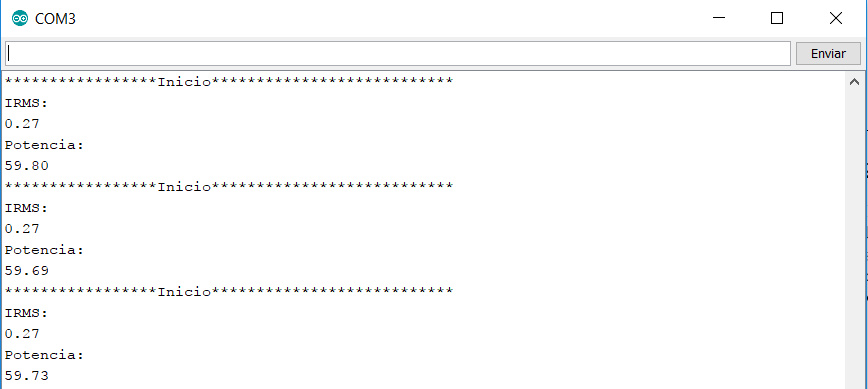
\includegraphics[scale=0.5]{imagenes/arduinoidemuestras.png}
	\caption{Monitor serial Arduino IDE.}
	\label{fig:monitorserial}
\end{figure}

\begin{figure}[H]
	\centering
	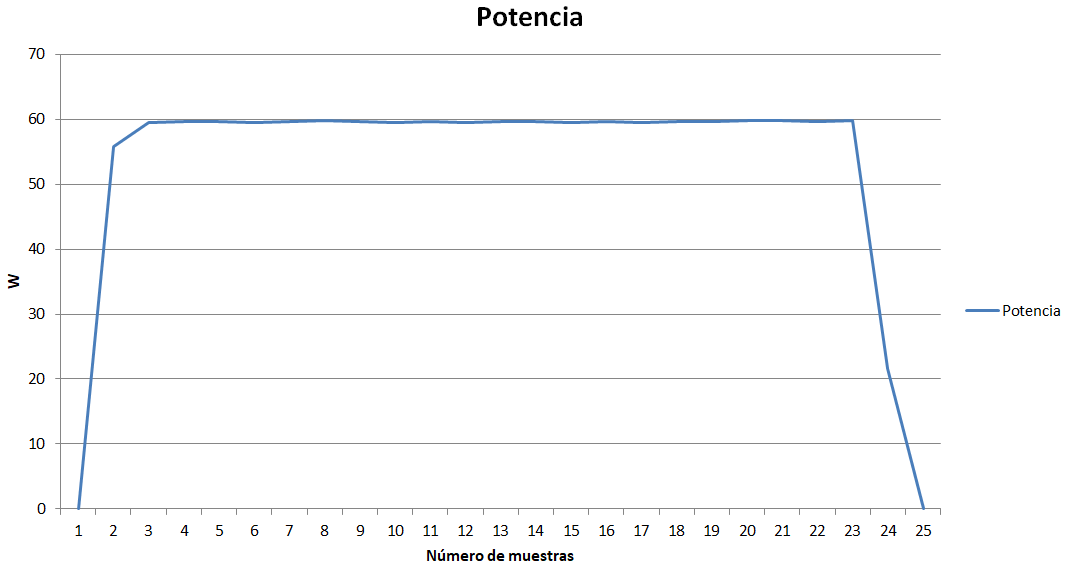
\includegraphics[scale=0.5]{imagenes/graficobombilla.png}
	\caption{Gráfico muestras recogidas.}
	\label{fig:graficobombilla}
\end{figure}

\section{Prueba con un electrodoméstico real}

Para esta prueba se ha conectado el sensor a un congelador y se han recogido medidas durante la noche obteniendo los siguientes resultados (\ref{fig:graficocongelador}). Además podemos observar como justo en el momento en el que el compresor del congelador vuelve a conectarse (Cuando detecta que ha perdido demasiada temperatura) el consumo se dispara ya que al volver a conectarse es cuando más energía consume.

\begin{figure}[H]
	\centering
	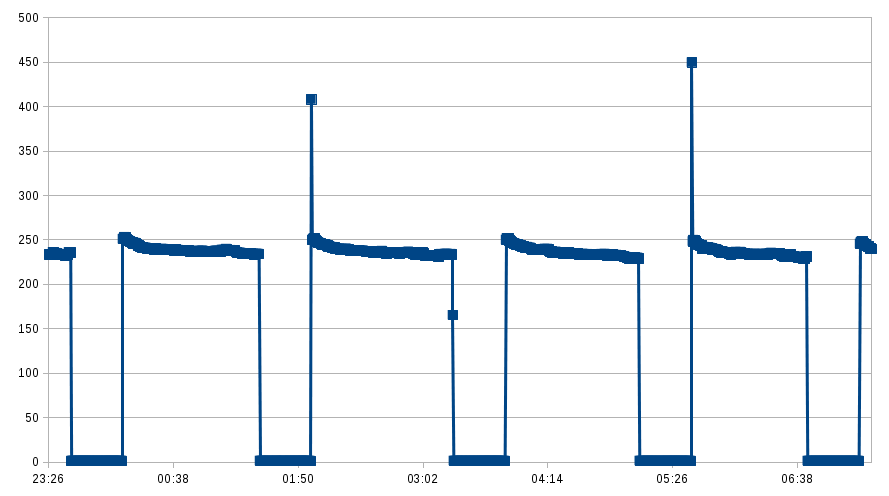
\includegraphics[scale=0.5]{imagenes/graficoFrigo.png}
	\caption{Muestras recogidas congelador.}
	\label{fig:graficocongelador}
\end{figure}

 Si analizamos los resultados más en detalle vemos que donde se produce un cambio significativo de la potencia registrada corresponde al tiempo que el compresor del congelador está activo y el tiempo que está apagado siempre es el mismo, como podemos ver con estos datos obtenidos directamente:

\begin{table}[H]
	\centering
	\begin{tabular}{|l|l|l|c|}
		\hline
		Hora                     & Medida   & Estado & \multicolumn{1}{l|}{Duración} \\ \hline \hline
		31/08/2017  23:39:12  AM & 1.23     & Off    & \multirow{2}{*}{0:29}         \\ \cline{1-3}
		01/09/2017 0:08          & 1.20     & Off    &                               \\ \hline
		01/09/2017 0:08          & 250.90   & On     & \multirow{2}{*}{1:35}         \\ \cline{1-3}
		01/09/2017 1:27          & 234.00   & On     &                               \\ \hline
		01/09/2017 1:27          & 1.21     & Off    & \multirow{2}{*}{0:30}         \\ \cline{1-3}
		01/09/2017 1:57          & 1.19     & Off    &                               \\ \hline
		01/09/2017 1:57          & 408.01 W & On     & \multirow{2}{*}{1:22}         \\ \cline{1-3}
		01/09/2017 3:19          & 165.26 W & On     &                               \\ \hline
		01/09/2017 3:19          & 1.20 W   & Off    & \multirow{2}{*}{0:30}         \\ \cline{1-3}
		01/09/2017 3:49          & 1.19 W   & Off    &                               \\ \hline
		01/09/2017 3:49          & 250.04 W & On     & \multirow{2}{*}{1:17}         \\ \cline{1-3}
		01/09/2017 5:06          & 229.31 W & On     &                               \\ \hline
		01/09/2017 5:07          & 1.20 W   & Off    & \multirow{2}{*}{0:29}         \\ \cline{1-3}
		01/09/2017 5:36          & 1.19 W   & Off    &                               \\ \hline
		01/09/2017 5:37          & 449.66 W & On     & \multirow{2}{*}{1:06}         \\ \cline{1-3}
		01/09/2017 6:43          & 231.48 W & On     &                               \\ \hline
		01/09/2017 6:44          & 1.19 W   & Off    & \multirow{2}{*}{0:29}         \\ \cline{1-3}
		01/09/2017 7:13          & 1.18 W   & Off    &                               \\ \hline
		01/09/2017 7:14          & 245.68 W & On     & \multicolumn{1}{l|}{}         \\ \hline
	\end{tabular}

	\caption{Tabla datos}
\label{fig:datoscongelador}
\end{table}
Todos estos resultados han sido obtenidos sin abrir en ningún momento la puerta del congelador. Pero en caso de que se abra la puerta del congelador se perderá frío y tendrá que conectar el compresor antes como podemos ver en esta otra gráfica (\ref{fig:abriendopuerta}) en la que justo en el momento en el que el compresor del congelador se apagó, se dejó abierta la puerta hasta que a los 3 minutos el congelador encendió de nuevo el compresor.

\begin{figure}[H]
	\centering
	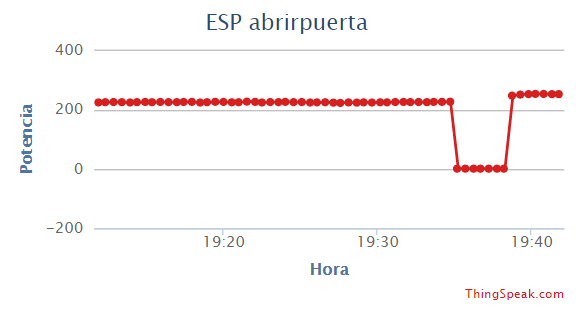
\includegraphics[scale=0.7]{imagenes/abriendopuerta.png}
	\caption{Muestras recogidas congelador.}
	\label{fig:abriendopuerta}
\end{figure}

\section{Posibilidades de explotación de un dispositivo como el presentado}

Como hemos visto gracias a la prueba anterior realizada en el congelador gracias a los patrones de consumo que observamos podemos determinar que electrodoméstico o dispositivo es el que está realizando esos consumos. Pero este estudio de los datos de consumo recogidos podría ir a más ya que como hemos observado es posible incluso determinar cuando el usuario ha abierto la puerta del congelador, esta idea puede ser aplicada en otros muchos electrodomésticos. De esta forma podrían extraerse patrones de comportamiento del usuario basados en los consumos de sus electrodomésticos permitiendo saber por ejemplo a que hora suele comer (basado en los cambios de consumo tanto de la vitrocerámica como el frigorífico) o si esta persona se encuentra o no en su hogar basándonos en el consumo eléctrico que se esté realizando en relación con la hora del día que sea.

Esto nos lleva a pensar que una empresa que estuviese interesada en recopilar datos a cerca de los hábitos de consumo de la población como puede ser Google o cualquier otra empresa, podría viendo los datos recogidos detectar que electrodoméstico o aparato eléctrico está en ese momento consumiendo electricidad y podría informar al usuario por ejemplo de cuantas luces tiene encendidas en ese momento en su casa, si está encendido el televisor, etc. Se podrían reducir en gran medida los costes de este dispositivo fabricándolo en masa.